% Straight up stealing preamble from Eli Holmes 
%%%%%%%%%%%%%%%%%%%%%%%%%%%%%%%%%%%%%%START PREAMBLE THAT IS THE SAME FOR ALL EXAMPLES
\documentclass{article}

%Required: You must have these
\usepackage{Sweave}
\usepackage{graphicx}
\usepackage{tabularx}
\usepackage{hyperref}
\usepackage{natbib}
\usepackage{gensymb}
%\usepackage[backend=bibtex]{biblatex}
%Strongly recommended
 %put your figures in one place
 
%you'll want these for pretty captioning
\usepackage[small]{caption}

\setkeys{Gin}{width=0.8\textwidth} %make the figs 50 perc textwidth
\setlength{\captionmargin}{30pt}
\setlength{\abovecaptionskip}{0pt}
\setlength{\belowcaptionskip}{10pt}
% manual for caption http://www.dd.chalmers.se/latex/Docs/PDF/caption.pdf

%Optional: I like to muck with my margins and spacing in ways that LaTeX frowns on
%Here's how to do that
 \topmargin -2cm     
 \oddsidemargin -0.04cm   
 \evensidemargin -0.04cm  % same as oddsidemargin but for left-hand pages
 \textwidth 16.59cm
 \textheight 22.94cm 
 %\pagestyle{empty}       % Uncomment if don't want page numbers
 \parskip 7.2pt           % sets spacing between paragraphs
 %\renewcommand{\baselinestretch}{1.5} 	% Uncomment for 1.5 spacing between lines
\parindent 0pt% sets leading space for paragraphs
\usepackage{setspace}
%\doublespacing

%Optional: I like fancy headers
\usepackage{fancyhdr}
\pagestyle{fancy}
\fancyhead[LO]{Do climate change experiments actually change climate?}
\fancyhead[RO]{2017}
 
%%%%%%%%%%%%%%%%%%%%%%%%%%%%%%%%%%%%%%END PREAMBLE THAT IS THE SAME FOR ALL EXAMPLES

%Start of the document
\begin{document}

% \SweaveOpts{concordance=TRUE}
 \bibliographystyle{/Users/aileneettinger/citations/Bibtex/styles/nature.bst}
\title{How do climate-change experiments actually change climate?} % Paper 1/Large group paper from Reconciling Experimental and Observational Approaches for Climate Change Impacts %Aaron suggests "Do climate-change experiments actually change climate?" for a title.
\author{A.K. Ettinger,I. Chuine, B.I. Cook, J.S. Dukes, A.M. Ellison, M.R. Johnston, A.M. Panetta,\\ C.R. Rollinson, Y. Vitasse, E.M. Wolkovich}
%\date{\today}
\maketitle  %put the fancy title on
%\tableofcontents      %add a table of contents
%\clearpage
%%%%%%%%%%%%%%%%%%%%%%%%%%%%%%%%%%%%%%%%%%%%%%%%%%%

\section* {Abstract}
\par Experiments that alter temperature and precipitation (e.g., with infrared heaters, rain shields, and supplemental watering) are critical tools that scientists use to understand and forecast the biological effects of climate change. We argue here that these experimental results may be interpreted in misleading ways, however. The common practice of summarizing and analyzing only the mean changes in temperature and precipitation across treatments hides potentially important variation in treatment effects over space and time. Furthermore, there are often unintended secondary treatment effects, such as soil drying in conjunction with warming, which are rarely fully explored and are likely to have important biological consequences. We demonstrate these points using daily climate data from 12 field-based climate change experiments that use active warming methods. Based on our findings, we make recommendations for future experimental design, analysis, and data sharing that we believe will improve the ability of climate change experiments to accurately identify and forecast species' responses to changes in climate.
\section* {Introduction}
\par Climate change is dramatically altering Earth's biota, increasingly shifting the physiology, distribution, and abundance of organisms, and causing cascading community and ecosystem effects \citep{shukla1982,cox2000,thomas2004,parmesan2006,field2007,sheldon2011,urban2012}. Much uncertainty remains, however, about how particular individuals, populations, species, communities, and ecosystems will respond as shifts in temperature and precipitation regimes become more extreme. Predicting these biological responses to current and future climatic change, and how they will feedback to affect earth's climate and ecosystem services, are among the most significant challenges facing scientists today.

% EMW - shorten and move (could fit as a clause right before your first section where you say what we focused on): Much work has focused on temperature because increased greenhouse gas emissions have relatively straightforward effects on it, relative to precipitation \citep{ipcc2013}. Christy: I think a big part is also that we’re a lot more confident that things are going to get warmer in most places whereas precipitation is very hard to predict and the directionality will have a lot more spatial variability. I'm not sure you need to mention this (it could just be a rabbit hole), but if you do, I htink you can just cite IPCC for the spatial patterns.

\par Field-based experiments that alter temperature and precipitation are critical for identifying causal effects of climate change on biological systems \citep[e.g.,][]{box1978,williams2007,gelman2014}. Researchers use a variety of other strategies to understand and forecast biological responses, including observational studies and model-based approaches, but these other strategies alone are insufficient for several reasons. Observational studies, which typically correlate recorded biological patterns with measured trends in climate, are insufficient because it is impossible to disentangle the causal effects of warming from other factors, such as successional stage or land use, that have also changed.%Christy thinks this is too vague: I think this is too vague… do you want to narrow down on one example like phenology or species distributions? 
 Performance of process-based models, which rely on explicit empirical relationships between observed phenomena and climate, can be limited because the underlying assumptions of these models may be poorly constrained \citep [e.g.,][]{pearson2004,ibanez2006,swab2012}. 
In addition, both of these approaches are challenged by the fact that future change is expected to result in conditions that fall outside the range of historical variability and well beyond what  \citep{ohlemuller2006,williams2007,williams2007b,ipcc2013}.  %Aaron: Is it necessary to define historically? Does it mean since climatic records begin in the 1880s? Or temperature reconstructions through the Holocene? Or when Homo sapiens has existed as a species. 
%a recent NCC paper described it this way: "The rate of warming over the past 50 years (0.13 °C ± 0.03 °C per decade) is nearly twice that for the previous 50 years5, and the global temperature by 2100 is likely to be 5–12 standard deviations above the Holocene mean6."
Experiments can create these ``no-analog" climate scenarios forecasted for the future, particularly when they employ active warming methods, such as gas-powered forced air heaters, electrical-powered soil warming cables, or infrared heaters \citep{shaver2000,williams2007b,aronson2009}. Active warming is often combined with precipitation manipulations (e.g., snow removal, water additions, or water reductions), and can isolate effects of temperature and precipitation from other environmental changes.\citep [e.g.,][]{price1998,cleland2006,sherry2007,rollinson2012}. In addition, if regression designs are used [e.g.,][]{pelini2011}and a range of warming and precipitation treatments are applied, non-linear responses can be estimated. Compared with controlled indoor growth-chamber experiments, field-based experiments offer the possibility of preserving important, but unknown or unquantified feedbacks among biotic and abiotic components of ecosystems. 
\par These experiments are a powerful tool, used to draw conclusions about how climate change will affect species' performance (e.g. growth and survival) and distributions \citep{dukes1999,hobbie1999,reich2015,gruner2016}. But is it reasonable to extrapolate experimental findings from these experiments to the real world? Do they actually alter climate in the ways that we think they do? There is reason to suspect they they do not: previous work suggests that experimental climate manipulations do not alter climate in ways that are consistent with observed changes in climate over time \citep{wolkovich2012}. However, most climate change experiments summarize and interpret only the mean effect of their climate manipulations. A detailed assessment of how active warming experiments alter the climatic conditions experienced by organisms, and the extent to which these conditions are similar to current field conditions or anticipated climate change, is lacking. 
\par We investigate if and in what ways climate change experiments actually change climate, beyond simple mean shifts. We use plot-level daily microclimate data from 12 active warming experiments to illustrate the direct and indirect ways that climate is altered by experimental manipulations, beyond simple shifts in the mean. We highlight the challenges associated with quantifying and interpreting experimental shifts in climate and the biological responses to these climatic manipulations, given that manipulations alter more than mean values. Finally, we use findings from our synthesis to make recommendations for future climatic change experiments (Box 1). We focus on in situ active warming manipulations, because recent analyses indicate that active warming methods are the most controlled and consistent \citep{kimball2005,kimball2008,aronson2009,wolkovich2012}. The data we use were collected between 1991 and 2014 from North American and European climate change experiments (Figure \ref{fig:map}) and have been merged into a new, publicly available Climate from Climate Change Experiments (C3E) database (see Supplemental Materials for details). 
%For supplement: we carried out a full literature review to identify all active field warming experiments then obtained daily (or sub-daily) climate data from as many as possible (we obtained data for 12/XX total identified experiments, see Supplemental Materials for details). We are thus able to show, for the first time, the complex ways that climate is altered by active warming treatments, both directly and indirectly. 
\section* {Complications in interpreting experimental climate change}
or 
\section* {Effects of experimental warming on local climate variables}
Climate change experiments often include detailed monitoring of climate variables at the plot level, yielding large amounts of data, such as daily or hourly temperature and other climate variables, over the course of the experiment. However, biologists generally are interested in the biological responses associated with each treatment (e.g., community dynamics; species' growth, abundance, or phenology). Not surprisingly, then, authors typically provide detailed information on the observed biological responses, but report only the mean change in climate over the course of the experiment and whether it matched their target level of change \citep[e.g.][]{price1998,clark2014a,clark2014b,rollinson2012}. Though the published focus is often on shifts in the mean, the imposed climate manipulations actually result in much more complex shifts. The magnitude of change in these manipulations may vary in time and space, and environmental conditions are often unintentionally altered by the presence of the experimental equipment itself. All of these complications challenge our interpretation of how experimental warming studies can be applied to forecast effects of climate change, and we discuss them in more detail below.
%CRR: I think it's good that you mention we don't report the climate because we're interested in the organisms and it leads to a publication bias. I don't know how to phrase it, but we (people that did the experiments) also often don't go into more detail because the experimental application can be very buggy with sensors going out, power outages, etc. and we've had to find that balance between accurately reporting our ecological story without going into the endless pits of study caveats.

\subsection* {Effects on local climate vary over time and space}%formerly "Treatments vary over time and space"
Reporting only the mean temperature difference across the duration of the study hides potentially important variations in daily, seasonal, and annual temperatures among treatments. Using the studies included in the C3E database, we found that active warming altered both above-ground and soil diurnal temperature ranges (DTR) in experimental plots, compared with control plots. We observed decreased DTR in above-ground temperatures with active warming compared with controls, perhaps because warming affected maximum temperatures less so than minimum temperatures. We found that active warming increased daily minimum air temperature by, on average, 0.84\degree C per degree of warming target, whereas maximum temperature increased only an average of 0.51\degree C per degree of target warming (Supplement). This may be similar to what is projected for parts of the world, since DTR is expected to be altered; however, changes in the DTR will likely vary spatially, as some regions have experienced greater daytime warming than nighttime warming, whereas others have experienced the opposite \citep{ipcc2013}. 
\par In addition to daily fluctuations, there are frequently strong seasonal and annual variations in experimental warming effects (Figure \ref{fig:effwarm}, \ref{fig:blockyear}). Seasonal variation may occur because treatments are not applied consistently over the year, either because heat applications are frequently shut off during winter months or because some heating methods, even if left on throughout the year, are not capable of applying consistent warming year-round \citep[e.g.][]{clark2014a,clark2014b,hagedorn2010}. For example, seasonal precipitation patterns can alter the effectiveness of warming treatments, since both infrared heaters and soil cables may fail to achieve the target temperatures during rainstorms \citep{peterjohn1993,hoeppner2012}. Wind also has been shown to alter thermal efficiency of infrared heaters, so if heater capacity is limited, target warming levels may not be reached during windy conditions \citep{kimball2005,kimball2008}. Thus, the dramatic inter-annual variation in the amount of effective warming (Figure \ref{fig:blockyear}) may arise from interactive effects of warming treatments and precipitation, wind, or other aspects of weather that vary annually, as well as seasonally. 
\par Treatment effects also vary spatially, adding Adding further complication to interpreting effects of climate change experiments. The C3E database contains three studies that used blocked designs, allowing us to examine spatial variation in the amount of warming (i.e. the difference between treatment and control plots within a block). We found that the amount of warming varied by more than one degree among blocks (Figure \ref{fig:blockyear}, Table 1S); lower warming treatments differed by over 60\% of their target temperature and higher warming treatments differed by over 100\%.
\par There are numerous potential causes for these differences in warming levels among blocks, given the same warming treatment. Fine-scale variation in vegetation, slope, aspect, soil type, or other factors can alter wind or soil moisture, which in turn affect the thermal efficiency of heaters or other aspects of the warming treatment \citep{peterjohn1993,kimball2005,kimball2008,hoeppner2012,rollinson2015}. The observed differences in effective warming among blocks highlight the importance of quantifying temperature, soil moisture, and other climate variables at the plot scale, and perhaps within plots, as well. 

\par It is, of course, unrealistic to expect experimental treatments to always be consistent one hundred percent of the time, at all spatial scales. In addition, there is bound to be variation in the amount of warming at daily, seasonal, and annual scales, as well as across space, as climate change progresses. Indeed, warming rates to date have varied over space and time \citep{ipcc2013}. However, fine-scale spatial and temporal variations in warming treatments are rarely analyzed explicitly, so the implications for interpretation of experimental findings are unclear. %In addition, it is unknown how the scale and magnitude of variation in experimental warming may differ from observed spatial and temporal variation in warming to date, as well as what will be experienced with future climate change.
% CRR: Is this seasonal precip pattern related to the point about snow cover you mention earlier? I'm wondering if there's some sort of snow or climatic threshold where warming has less of an impact. AKE: Could look seasonally at amount of warming to get at this...
%Jeff: I recommend cutting this (The scale is different than what we’re considering, so I think it sets the reader up for confusion). Accurate extrapolation of climate change experiments may depend on the extent to which experiments encompass a representative amount of existing natural variation (e.g., gradients in slope and aspect) present at the scale at which the extrapolation is being made. Spatial variation within experimental warming treatments and the absence of a direct space-for-time substitution adds complexity to extrapolations from experimental results \citep{johnson2008,jochner2013}.
\subsection* {Experimental infrastructure alters local climate}
The experimental structures themselves alter temperature and other important biotic and abiotic variables, in ways that are not generally examined or reported in experimental climate change studies. The importance of having appropriate controls that mimic a treatment procedure without actually applying the treatment is widely acknowledged in biology \citep[e.g.,][]{spector2001,johnson2002,quinn2002}. Though some researchers install treatments with non-functional warming equipment (`sham controls' or `disturbance controls') in experimental climate change studies, the magnitude and implications of structural effects on climate are rarely discussed or interpreted.
\par To investigate the magnitude of infrastructure effects, we compared temperature and soil moisture data from five active warming studies at two sites: Duke Forest and Harvard Forest \citep{farnsworth1995,clark2014a, marchin2015, pelini2011}. These were the only studies in our database that monitored climate in two types of control plots: structural controls (i.e., `shams' or `disturbance controls,' which contained all the warming infrastructure, such as soil cables or infrared heating units but with no heat applied) and ambient controls with no infrastructure added (see Supplemental Materials for details). Other studies monitored environmental conditions in only structural controls (n=3) or only ambient controls (n=4).
%Is it worth pointing out the long history of such "cage controls" in marine intertidal and subtidal research that somehow has not translated to terrestrial research? Or would that be overkill? 

\par We found that experimental structures altered above-ground and soil temperatures in opposing ways: above-ground temperatures were higher in the structural controls, compared with ambient conditions with no structures installed, whereas soil temperatures were lower in the structural controls compared with ambient soil (Figure \ref{fig:shamamb}a,b). This general pattern was consistent across the different temperature models we fit (mean, minimum, and maximum temperatures), although the magnitude varied across seasons (Figure \ref{fig:shamamb}a,b), as well as among studies, years, and with ambient temperature (Table XS). In addition, soil moisture was lower in structural controls compared with ambient conditions (Figure \ref{fig:shamamb}c). 
\par There are several possible reasons for the observed differences between ambient and structural controls. Infrastructure materials may shade the plots, reduce airflow, reduce albedo relative to surroundings, or otherwise change the energy balance. Structures could also interfere with snow accumulation, thereby reducing snowpack and its insulation. This likely plays a bigger role in soil temperature differences at the Harvard Forest sites (exp04, exp07), where average snowfall is over one meter, than at Duke Forest, where average snow accumulation is 20 cm or less. Although we could find very little discussion of measured temperature (or other) differences between ambient and structural control plots in most previously published work \citep[e.g.,][]{farnsworth1995,pelini2011,clark2014a,clark2014b}, Clark \textit{et al.} (2014) do mention that ``control of the air temperature was less precise, in part due to air scooping on windy days." Marchin \textit{et al.} (2015) also note that structural controls had mean spring air temperatures about 0.5 \degree C or more above ambient temperatures. Peterjohn \textit{et al.} (1994) reported cooler soil temperatures in structural versus ambient control plots, but only at shallow soil depths (4 cm deep, in their study). Similarly, in our analysis we found the greatest difference between soil temperature in sham and ambient controls to be in exp10, one of the two studies in which temperature was measured at depths of 2 cm (the other was exp07), rather than 15 cm deep (exp03 and exp04). 
\par In addition to the structural effects that we document here on temperature and moisture, experimental structures may alter conditions by altering herbivory and other biotic interactions \citep{kennedy1995,moise2010,wolkovich2012,hoeppner2012}. Most warming experiments to date deal with this by calculating focal response variables relative to ambient controls to account for the infrastructure effects \citep [e.g.,][]{marchin2015}. Further documentation and analysis of the effects on abiotic and biotic factors, as well as in depth interpretation of how these effects may alter focal variables, is an important next step for climate change experimentation, particularly if we wish to apply results to forecasting.

\section* {Secondary effects of climate change manipulations}
Climate change experiments often seek to manipulate one or two climate variables, such as temperature and precipitation. However, non-target abiotic and biotic factors may also be affected by these manipulations. For example, precipitation treatments typically reduce temperatures in climate change manipulations \citep{sherry2007,rollinson2012,mcdaniel2014}. McDaniel et al. (2014) observed that a twenty percent increase in precipitation reduced mean hourly temperatures by 0.3 \degree C over the course of their two-year experiment. The magnitude of this effect can vary in space and time, however (Figure \ref{fig:effwarm}). 
\par In addition, experimental warming typically increases vapor pressure deficit and reduces soil water content (Figure \ref{fig:mois}) \citep[e.g.,][]{sherry2007,morin2010,templer2016}. Of the twelve experiments in the C3E database, ten measured and reported soil moisture, and six measured air temperature in addition to soil moisture. % Chisty:I think some of this information was necessary earlier to help understand whenever only a subset of experimetns is shown
To examine the effects of air temperature on soil moisture, we applied linear mixed effects models to these six sites in C3E (see Supplement for details). .
We found that soil moisture was reduced by 0.2 percent, on average, per degree of air warming (Table XS). While active warming experiments often do not manipulate soil moisture directly, soil moisture is unavoidably affected by changing temperatures. 
\par Warming and precipitation treatments, and their indirect effects on soil moisture and other abiotic factors can also alter the biotic environment, which in turn can produce additional secondary effects that alter climate. For example, Rollinson et al. (2012) reported that tree composition shifted after three years of warming and modified precipitation treatments. These shifts in composition may change competitive dynamics and, in turn, affect resource levels, such as moisture in the soil. In addition, given that warming reduces soil water content, it is likely to affect soil microbial communities, and therefore available nutrients as well \citep{mcdaniel2014,mcdaniel2014b}. The magnitude of all of these effects are also likely to vary in space and time; some may be transient whereas others may be more permanent. %Anne Marie: Community level work done in the RMBL warming meadow should be sited here- Harte et al. 2014, for example.nThis experiment has found a shift from forbs to shrubs, and the shift to shrubs has caused more rapid snowmelt but also a recovery of soil carbon.
%Could also add something about shrubs, which can also shade soil, and might be worth saying something more specific about how transient (or not) some of the resource limitation may be (e.g. nitrogen cycling) because some experiments (Harvard Forest, boreal warming in AK?) show very different patterns between first couple years and longer-term dynamics?

% EMW: These next two paragraphs could be condensed a lot. Also, you have a lot of for examples in the paper. Probably need to pick out your few favorites and drop the rest (plus most of the for examples seem biased to be the authors' for example so I would be especially judicious in leaving too many). 
\par It can be difficult to tease apart the specific abiotic and biotic drivers of climatic conditions in climate change experiments, but understanding the effects of an experimental treatment on these interrelated variables is critical when trying to determine mechanistic explanations for observed responses to warming. Even when experimental artifacts are introduced, if their effects are quantified they can be helpful in understanding how abiotic and biotic factors interact to affect physiology. For example, we can learn about the controls on stomatal conductance when the normal co-variance between temperature, humidity, and soil moisture is altered. 
\par The widespread presence of unintended secondary effects of climate change manipulations highlights the importance of measuring environmental conditions at the plot level, and of using these measurements in data analysis and interpretation of results. Many climate change experiments (seven of the 12 in the C3E database, for example) model warming and/or precipitation treatments as categorical predictors (and in some cases, orthogonal crossed treatments, when both treatments are included in the experiment, i.e. a traditional repeated measures, three-way ANOVA). The interacting and secondary effects of these manipulations, as well as the plot-level variation in warming effectiveness and effects of experimental structures on temperature and soil moisture that we discuss above, demonstrate a clear need for an alternative modelling approach to fully understand the experimental results. One option is to include the continuous climate data (e.g., plot-level mean temperatures), as a predictor of the focal response variable, such as phenological state or species density \citep [e.g.,][]{marchin2015, pelini2014}. A challenge with this approach is that much of the true variation in the climate is lost through aggregation (e.g., calculating mean annual or seasonal temperature), and the chosen method of aggregation affects both the mean and variance of the climate estimate \citep [e.g.,][]{clark2014b}. 
% EMW (cut): It may not be obvious which method of aggregation, or which combination of aggregated climate variables, is most appropriate, and this will likely depend on the response variable of interest. In these cases, model selection approaches have been used to identify the climate aggregation method that best explains the focal response\citep [e.g.][]{morin2010}. Alternatively, a continuous development model can be used to capture the full range of variation present in a climatic variable during the study period \citep [e.g.][]{clark2014b}.
\section* {Biological implications}
%In this section, it is important that we make strong links between the unreported statistics that we just described (seasonal and temporal variation, secondary effects) and potential biological responses.nI feel that as it is written right now, it is more a summary of just the biological responses with not enough emphasis on now they relate to better microclimate reporting.

%Aaron: This section is important, but it seems too large relative to the title and goal (what climatic change experiments do to climate) of the ms. The first paragraph seems right on, but the subsequent ones to me detract from the main message of the ms. Think about dropping them or condensing to one shorter paragraph. That will also make the transition to the next section a little smoother.
%Christy:I think a lot of the arguments here were also brought up in the “Secondary effects Section”… I we need to more clearly delineate what the secondary effects and then which are the biological implications of concern to streamline these two sections.

% EMW: The first and last sentence of this paragraph are awesome!
\par We have highlighted a suite of factors that complicate interpretations of warming experiments. We argue that these largely unintended alterations are important for scientists to fully understand and report in their research. This is especially important because unintended climate alterations are likely to have biological implications, including for many of the major responses studied in warming experiments, such as plant phenology (Figure \ref{fig:biolimp}). Intepretation of experimental climate change effects on biological responses may be misleading, because the intended climate treatments (i.e. categorical comparisons or target warming levels) are generally used as explanatory variables in analyses. The interpretation is likely to be altered by using fine-scale, measured climate as the explanatory variables (e.g., plot-level temperature and soil moisture), because detailed examination of multiple microclimate variables will allow a more complete understanding of the indirect, as well as direct, effects of applied treatments on abiotic and biotic drivers of focal responses.

\par Plant phenology may exemplify a biological response that is muted in experiments versus observational studies (Figure \ref{fig:biolimp}b). This is because phenology is likely to be altered in opposing ways by the direct effects of increased air temperatures---which generally advance phenology \citep{wolkovich2012}---and the indirect effect of decreased soil moisture---which may delay phenology or at least reduce advancement due to warming \citep{penuelas2004,craine2012,matthews2016}. %Aaron: This is true only for species whose phenological responses are cued by temperature (and/or moisture). How many species (what %age) is that? See Davis et al. 2015 AJB for some discussion. 
These opposing drivers may be responsible for the observed discrepancy between observational and experimental phenological responses to warming \citep{wolkovich2012}. Other biological responses may be exaggerated in experiments when direct and indirect effects of climate manipulations work in concert (Figure \ref{fig:biolimp}c). In both cases, accounting for indirect, as well as direct, effects of warming is critical for accurate interpretation about the consequences of climate change \citep{kharouba2015}. Since climate change experiments have indirect effects on the biotic as well as abiotic environment \citep{hoeppner2012,pelini2014,diamond2016}, a critical question is the extent to which these indirect effects are accurate forecasts of future shifts that are likely to occur with climate change, or due to side-effects that are unlikely to occur outside of experimental systems \citep{moise2010,diamond2013}.
%ADd this somewhere?\par stuff moved from variance: These differences in temperature range and variation, appear to be small, but they may be important. For example, even slight changes in temperature can alter critical biological thresholds, such as freeze-thaw cycles \citep{mcdaniel2014}. Other studies corroborate our findings that warming treatments may affect diurnal versus night temperatures differently \citep{shen2016,matthews2016}; these shifts can have critical biological effects. Leaf-out timing of temperate trees, for instance, respond three times more to daytime than to night- time temperature, so that maximum temperatures would have an overwhelming effects on spring phenology over minimum temperatures \citep{fu2016, piao2015}.n
\section* {Conclusions}
 \par Climate change experiments provide invaluable information about biological responses to climate change, yet the full range of changes in environmental conditions imposed by these experiments is rarely presented. We believe the data we have compiled in the C3E database, as well as the complications we have highlighted, provide a foundation for designing better experiments and gaining the most knowledge and utility from existing experiments. We also recognize that funding levels, time, and logistical issues often constrain researchers' abilities to monitor and analyze a larger suite of environmental conditions in climate manipulations.nHowever, we argue that these data have value for the broader research community, and that they should be collected and made public when possible. In Box 1, we describe specific recommendations to improve implementation, interpretation, and communication of the results of climate change experiments in the future.
 \par Researchers have been studying the implications of climate change for ecosystems for nearly four decades \citep[e.g.,][]{tamaki1981,carlson1982}.
Yet, as climate change across the globe continues with projected warming likely to exceed 2 \degree C over the next 80 years \citep{ipcc2013}, ecologists are challenged to not only document impacts but make quantitative, robust predictions. Our ability to meet this challenge requires building on the data from current and past experiments to better understand how changes in climate alter ecological processes, and to design better experiments in the future. To facilitate this, we have compiled the first database of fine-scale climate data from multiple warming experiments and shown how time, space, and experimental artifacts may hinder simple interpretations of climate change experiments. 

\par The next steps require the ecological community to evaluate their data in new ways and build on these data to develop and use novel approaches in future experiments. This will allow researchers to more accurately and confidently elucidate mechanisms underlying biological responses and feedbacks. %Jeff: Our “ask” might be worth rethinking. We might consider this as the beginning of a larger conversation..
\section* {Box 1: Recommendations for future climate change experiments} 
\begin{enumerate}
\item\textit{Include both structural and ambient controls} and collect, use, and report data collected within them. Fewer than half of the studies in our C3E database included these two control types and monitored climate and the focal biological response within them (5 out of 12); all experiments showed significant effects of infrastructure. Future consistent monitoring of all climate and biological variables in both control types will enable scientists to tease apart mechanisms due to experimental design from mechanisms due to shifts in climate. To date, these side effects are rarely reported or interpreted in climate change experiments, making them ``demonic intrusions" in need of ``eternal vigilance" to reduce \citep{hurlbert1984}. 
\item\textit{Maximize the length of climate change experiments} by running them for as long as possible. This will allow study of how inter-annual variations interact with climate change treatments, especially when looking at non-linear and multi-year processes such as phenology. It will also allow us to understand how long-term responses may differ from transient ones \citep{saleska2002,franklin1989,giasson2013,harte2015}. %Ben: I agree, obviously, but this leaves us open to criticisms about cost. Is there something we can say along the lines of, "better to allocate resources to more years of experiment rather than X"?
\item\textit{Collect and analyze fine-scale climate data} to allow for minimum and maximum values, as well as variance and critical thresholds, such as the number and duration of freeze-thaw events and accumulated chilling hours, to be analyzed and interpreted, in addition to mean values \citep{mcdaniel2014,vasseur2014}. Most data loggers already collect data every minute, and store 30-minute, hourly, or daily means. We suggest saving the raw data to allow quantification of variance (and other summaries) at different temporal resolutions. In assessing which frequency of measurements is most appropriate for analyses (e.g., hourly, twice daily), it is critical to consider the chronobiology of the event and organisms of interest. For ants, this might mean that temperatures be monitored at the frequency of minute \citep{shavit2017}; for bacteria, even more frequently. Although this recommendation requires large and potentially cumbersome data files, recent advances in data standards and remote-storage repositories make this a more feasible request now than when these warming experiments began.
\item\textit{Analyze measured climate variables rather than targets}. There can be substantial variation in the effects of warming and precipitation treatments among plots and across time (Figure \ref{fig:blockyear}). Furthermore, these applied climate treatments are not independent: precipitation treatments alter the effectiveness of warming, and warming treatments alter available moisture levels. Analyzing climate in this way will allow much more in-depth understanding of the drivers and the biological effects of variation in temperature and moisture.

\item\textit{Consult observational records and forecasts to design relevant manipulations}. If the goal is to mimic future climate conditions, careful consultation of climate change projections, as well as historical data, for the study region can aid in selection of warming and precipitation treatment methods that most closely mimic anticipated changes. When it is not possible or desirable to match anticipated changes in climate, studies should report how imposed treatments compare to projected changes and/or past observations \citep[see, e.g.,][]{hoover2014}. In addition, the timing of the imposed treatments should be carefully considered. If it is not possible or desirable to apply continuous treatments throughout the study, the seasonality and timing of treatments should be explicitly reported and the climate should be monitored throughout, even when no manipulations are implemented.

\item\textit{Publish high quality, usable data and metadata} such that data can easily be shared. Include detailed data about experimental treatments, such as the number and cause of missing data points for climate, the timing of applied warming treatments (i.e., exact start and end dates, within and across years). Given that experimental in situ active climate manipulations are logistically challenging and expensive \citep{aronson2009}, and that they often produce a large volume of fine-scale climate data, good curation and data sharing will ensure wider use and more in-depth understanding of these valuable data. When studying biological implications of a global challenge as large as climate change, it will facilitate progress if we can design, run, and report experiments in such a way that we can eventually create a global data set. We found that studies report a diverse range of climate variables, collected in different ways (Table 1). It is a challenge to synthesize these diverse data, and to tease apart whether variable findings are due to methodological differences, to measurement error, or to true variation in biological responses. 
%Table 1: Table summarizing different depths/units/measurements used with e.g., in the the C3E database, soil temperature was collected at depths ranging from 2 to 25 cm and soil moisture was collected at depths ranging from 8 to 30 cm, using different units and methods
\end{enumerate}
\bibliography{/Users/aileneettinger/citations/Bibtex/mylibrary}
\clearpage

\section* {Figures}

% Fig 4: Can you add the linear regression line to this? Helps make it easier to see deviance from 1:1 line ... perhaps force origin to 0,0? Not sure, to discuss.
\begin{figure}[p]
\centering
\includegraphics{../Analyses/maps/RadcliffeLocations_Experiments.png} 
\caption{Climate data from 12 climate change experiments in North America and Europe are included in the C3E database and analyzed here. See Supplemental Materials for details.} 
 \label{fig:map}
 \end{figure}
\clearpage
\begin{figure}[h]
\centering
 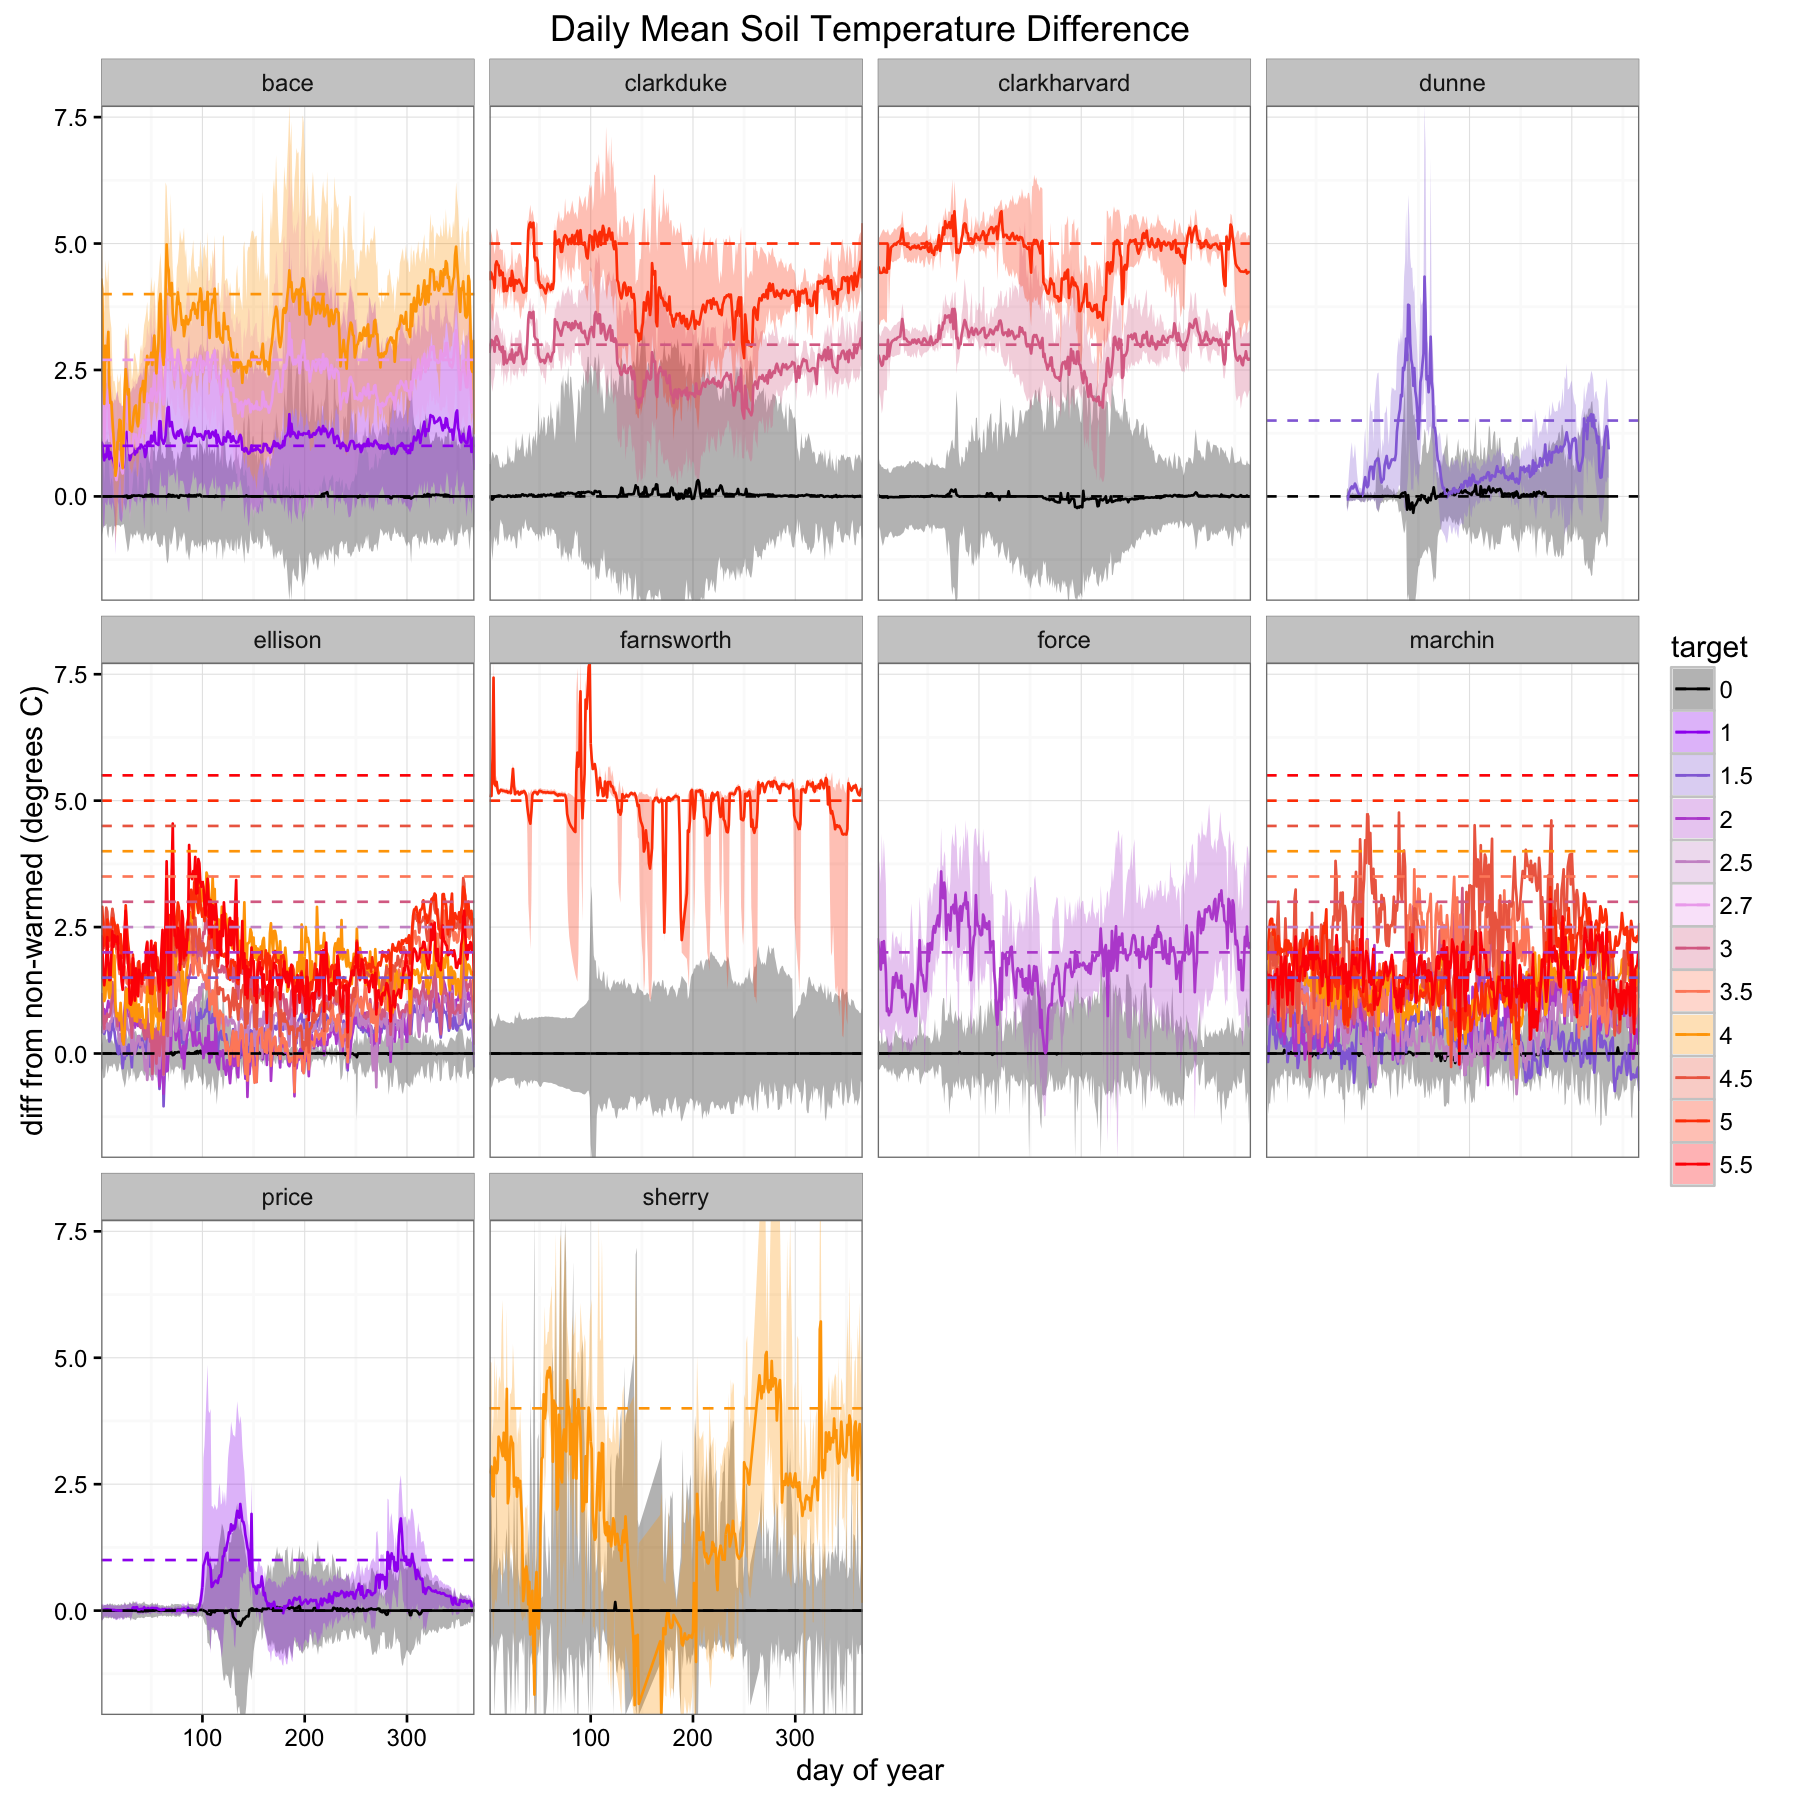
\includegraphics{../Analyses/figures/Exploratory_TimeSeries_SoilTemp1Mean_Deviation.png}
 \caption{Time series of deviations from mean soil temperature, in control (black line)
and warming treatments with various target warming levels (dashed lines) at 10 study sites.(The two sites not shown here did not monitor below-ground temperature). Daily temperature values were obtained by averaging across years for each day of the year for each plot in each study. We then averaged across plots to get the mean line and 95 percent confidence intervals (shaded areas, which therefore represent the variability in treatment effectiveness based on the replicates. Mean annual temperatures of the experimental site are shown in the upper right corner of each plot }
 \label{fig:effwarm}

 \end{figure}
 \begin{figure}[p]
   \centering
 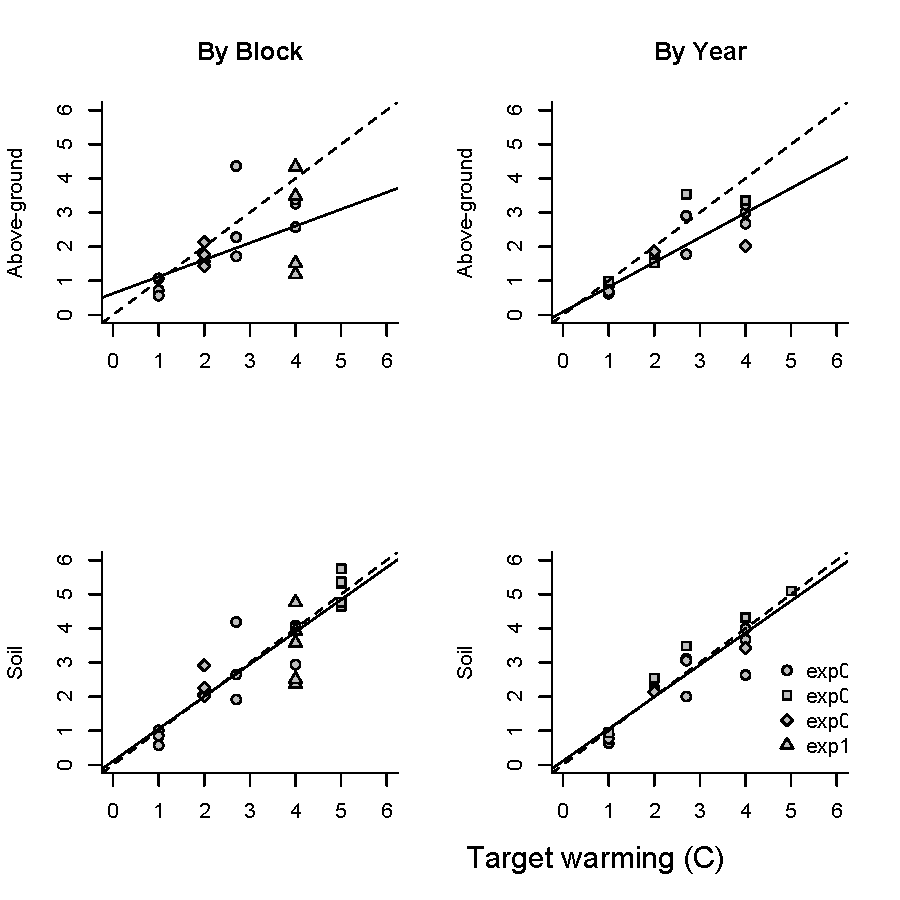
\includegraphics{../Analyses/figures/blockyearvar.pdf}  
 \caption{The amount of observed warming (i.e. the difference between treatment and control plots, within each block) varies among blocks (left panels), as well as among years (right panels). The solid line is the fitted relationship between target and observed warming, using a linear mixed effect model with a site random effect. The dashed line represents a 1 to 1 ratio (i.e. when observed warming is exactly equal to target warming). See Tables XS and XS for statistical differences. }%Christy: I like the simplicity of this figure, but I don’t understand what the groupings in this figure mean. I think we need to explain what experiments are being represented or at least characteristics in the caption… are these 3 the only ones that used block designs? What doe the “by year” mean – difference of a given plot relative to the total mean of the control?
 \label{fig:blockyear}

 \end{figure}
\clearpage





 \begin{figure}[p]
\centering
 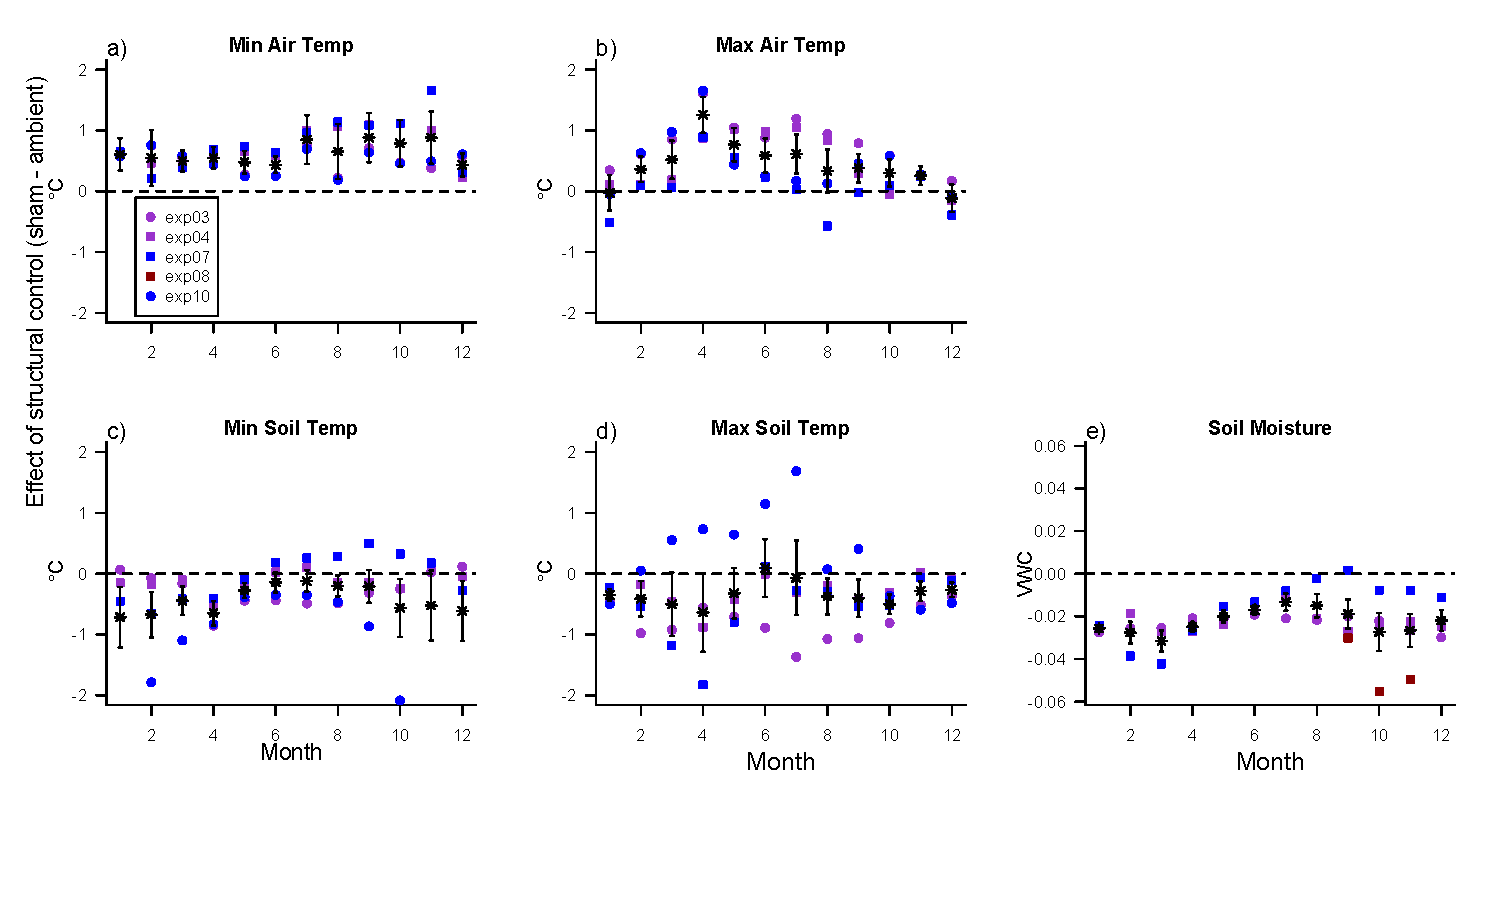
\includegraphics{../Analyses/figures/ShamVSAmbient_all.pdf}  
 \caption{Air temperatures were higher, whereas soil temperatures were lower, in general, in structural controls compared with ambient controls (i.e. with no control chambers or warming infrastructure in place). Soil moisture was lower in structural controls compared with ambient controls. We show fixed effects (in black) from a mixed effects model that accounts for differences in experimental design and other factors among sites with mixed effects model including site and year (nested within site) as random effects (see Table XS, Supplemental Materials for details). Site-level random effects are shown by symbols in blue (for those at Harvard) and pink (those at Duke).ADD letters to these panels?}
 \label{fig:shamamb}
 \end{figure}
\clearpage
 \begin{figure}[h]
    \centering
 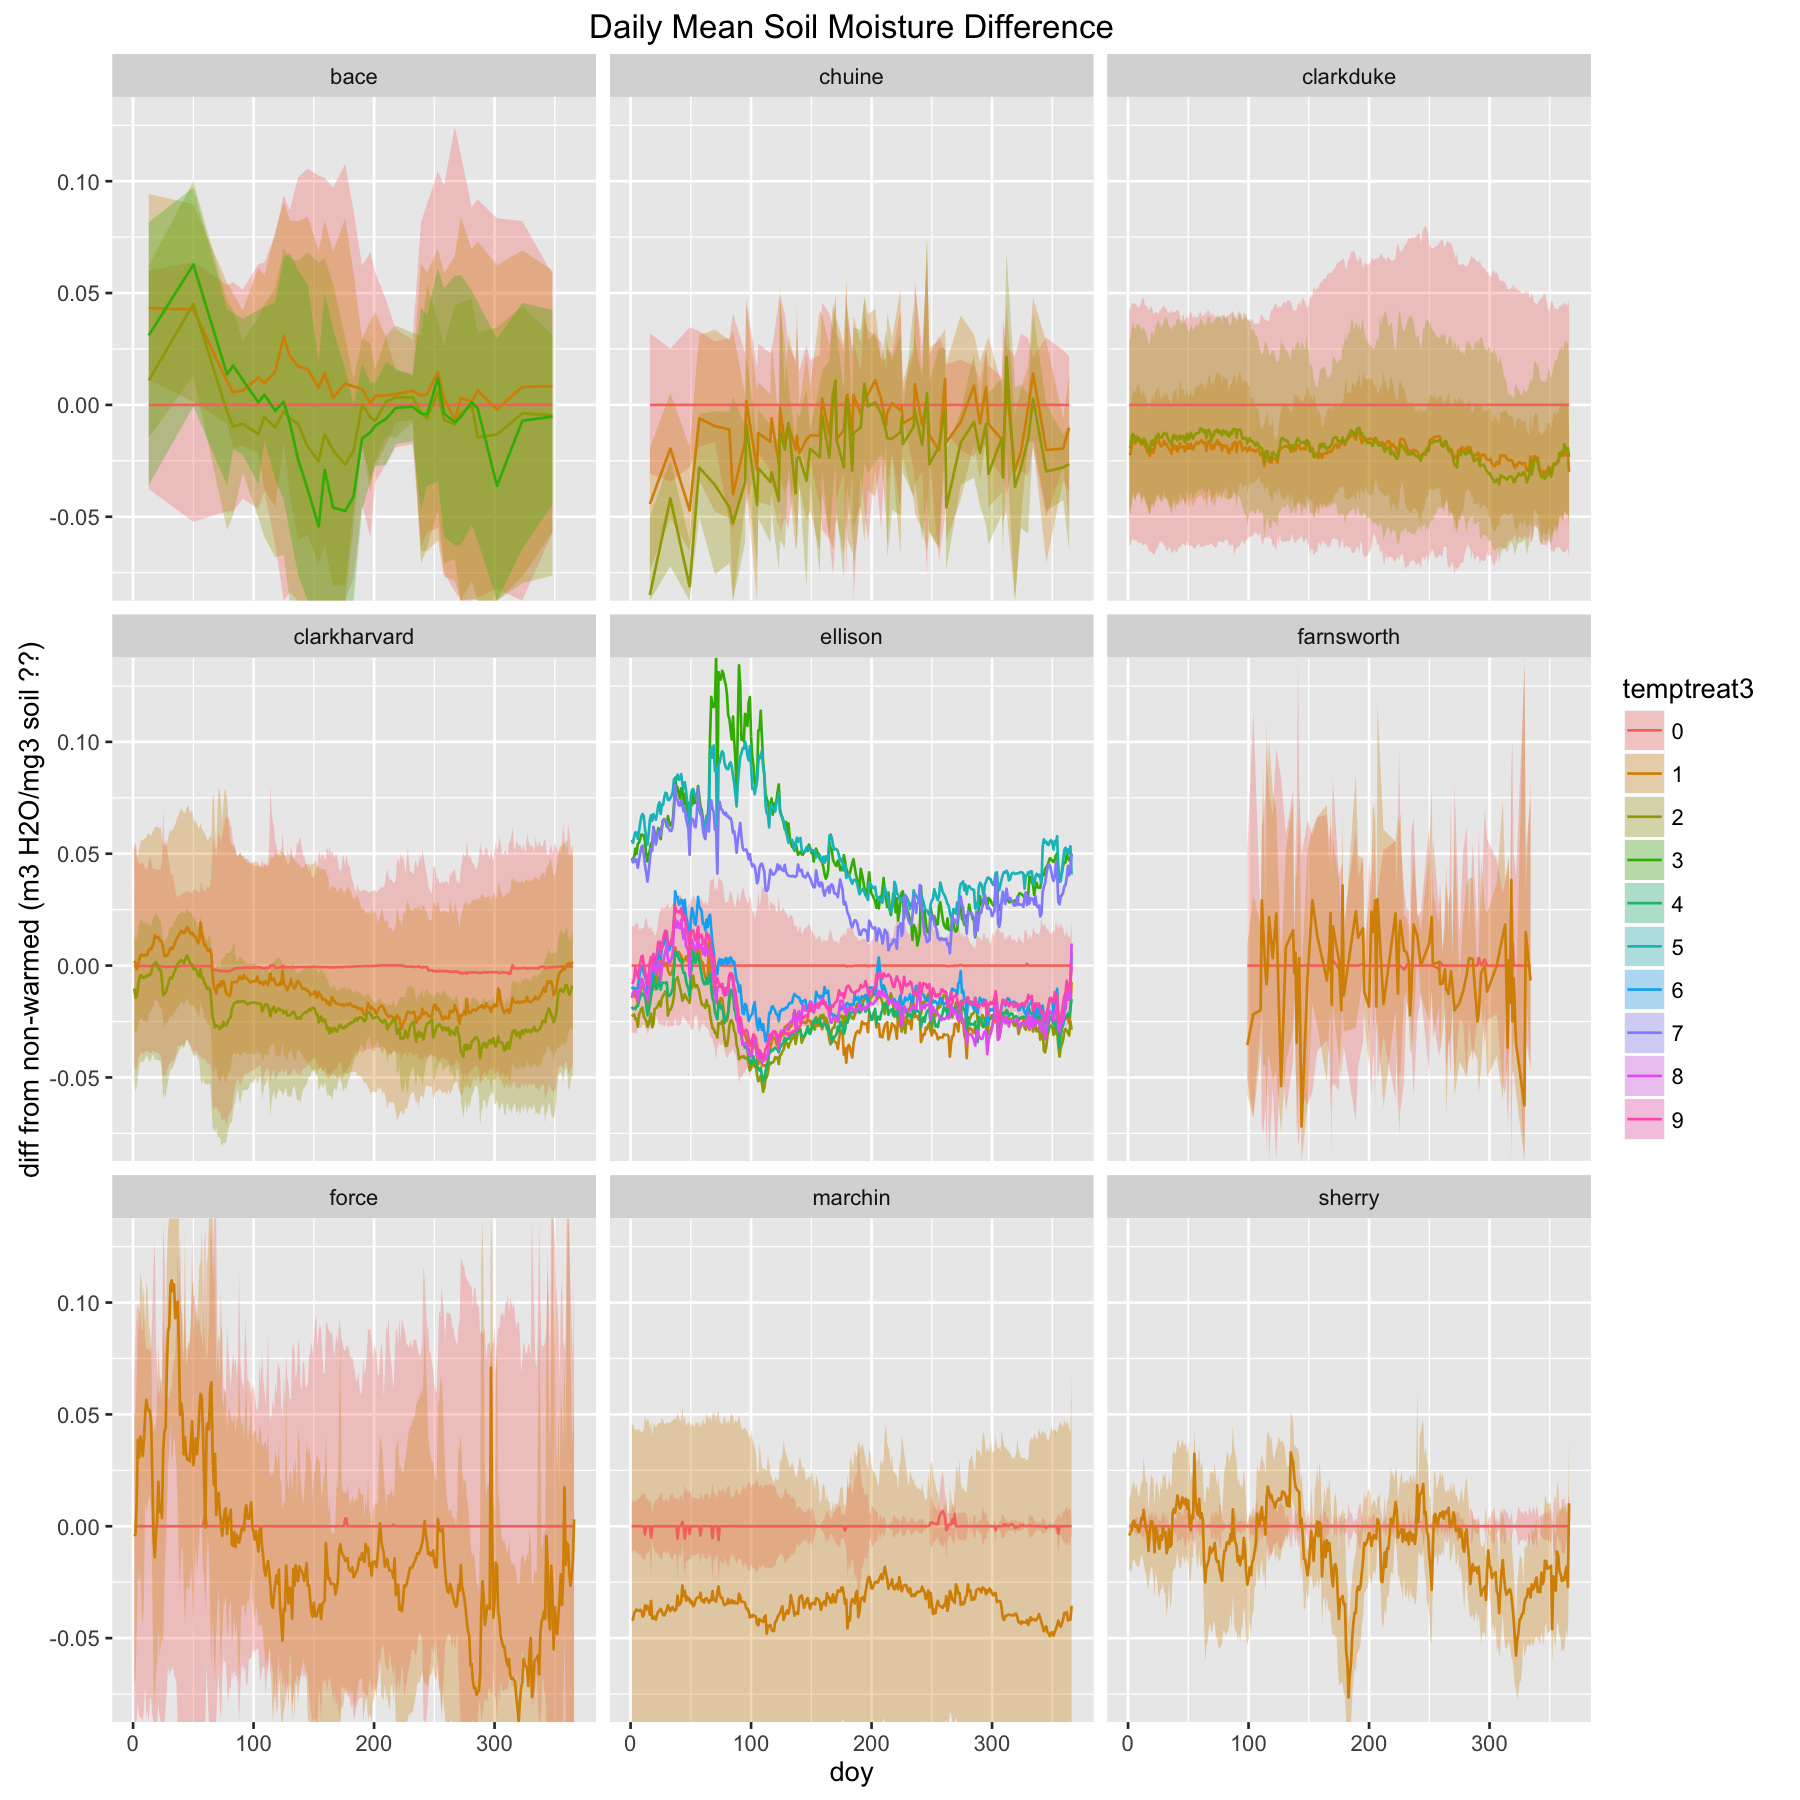
\includegraphics{../Analyses/figures/Exploratory_TimeSeries_SoilMoist_Deviation.png}  
 \caption{Time series of deviations from mean daily soil moisture in control (black line) and warming treatments with various target warming levels at 10 study sites.}
 \label{fig:mois}
 \end{figure}
 \clearpage
 \begin{figure}[h]
 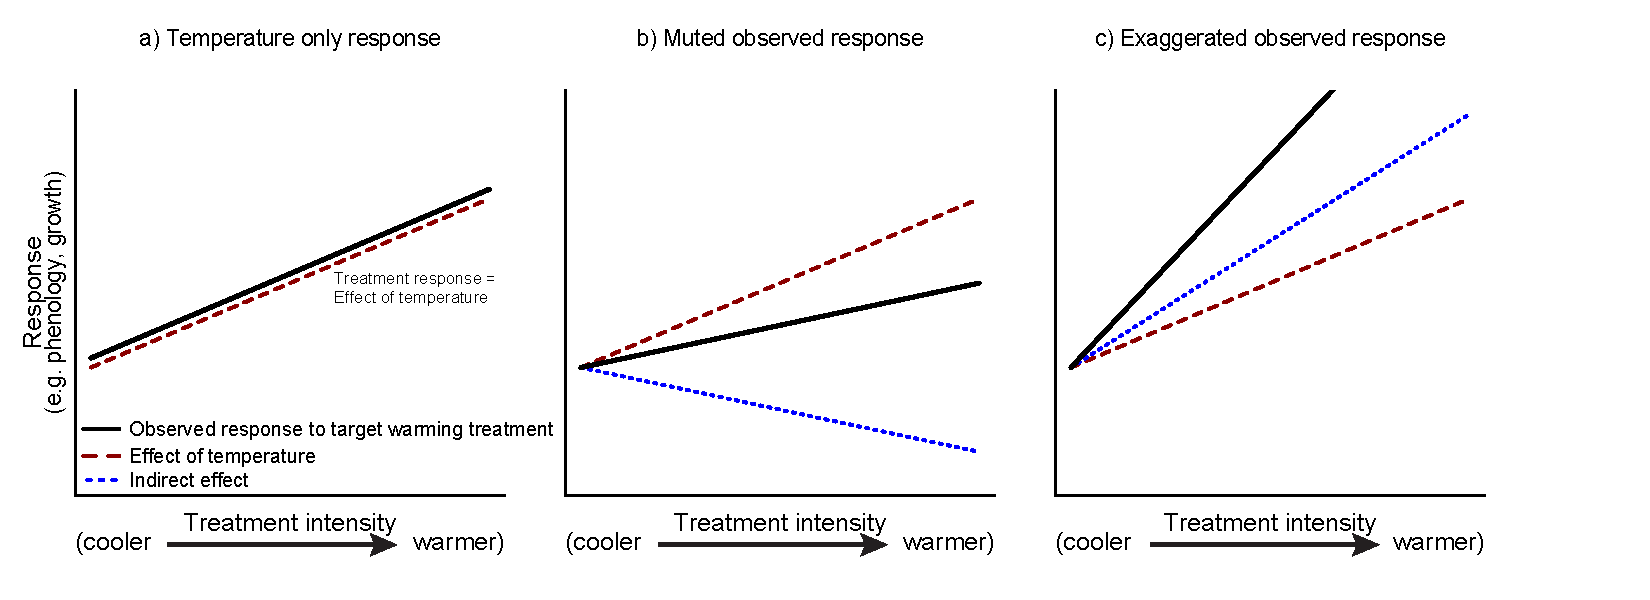
\includegraphics{../Analyses/figures/DirIndWarmingEffects.pdf} 
 \caption{Compared to direct responses to temperature alone (a), experimental warming may cause biological responses to be muted (b) or exaggerated (c), when indirect effects of experimental warming are also drivers of focal responses. For example, phenology, such as budburst which usually advances with warming, may appear to be less sensitive to warming in experiments versus observational studies \citep{wolkovich2012} because experimental warming reduces soil moisture and drying often delays phenology.}
\label{fig:biolimp}
  \end{figure}
%%%%%%%%%%%%%%%%%%%%%%%%%%%%%%%%%%%%%%%%
\end{document}
%%%%%%%%%%%%%%%%%%%%%%%%%%%%%%%%%%%%%%%%
